\documentclass[12pt,a4paper,twocolumn]{article}
\usepackage{amsmath}
\usepackage{amsthm}
\usepackage{amsfonts}
\usepackage{amssymb}
\usepackage{graphicx}
\usepackage{cite}
\usepackage{tikz}
\usetikzlibrary{arrows,shapes,automata,petri,shadows}
\usepackage[left=2cm,right=2cm,top=2cm,bottom=2cm]{geometry}

\newtheorem{myDef}{Definition}

\author{David Tamez, Josiah Hanna and Xiaorong Zhu}
\title{Evolving Petri Networks for High Level Robot Control}
\begin{document}


\maketitle

\begin{abstract}

Petri networks are mathematical models for representing dynamic systems. They have been applied to model high level robot control. In previous work, this has involved hand coding the Petri networks using the designers' knowledge of the target domain. While Petri nets provide a good tool for control and analysis of the robotics task, the hand coding is limitation for using large networks. In this paper we show how to use an evolutionary algorithm to automatically generate a correct Petri network for a specific task.

\end{abstract}

\section{Introduction}

Controlling robots depends on specifying actions on different levels of control. Control can be made easier by breaking a task down into component subtasks and then using these subtasks as the actions to plan with. Consider the task of a robots in the keepaway soccer domain. In this domain a team of robots must pass a ball amongst themselves while an advsersary robot tries to intercept the ball. At a low level a robot must control the exact angle and speed it is moving. However, it is easier for the robot to learn subtasks such as intercept the ball or kick ball and then plan using these subtasks as higher level actions \cite{whiteson}. Higher level action plans can be represented in different ways such as decision trees or neural networks. A third approach is to use Petri networks. 

A Petri net is a mathematical model representing a dynamic system. While decision trees and neural nets can be learned, previous work using Petri nets requires the nets to be hand designed for the task \cite{ziparo2011petri}. In this paper we demonstrate a method for automatically generating Petri nets using an evolutionary algorithm based on the Neuroevolution for Augmenting Topologies algorithm for evolving neural networks.

The layout of this paper is as follows. In section 2 we give background information on Petri networks and neuroevolution. Section 3 describes previous work on Petri nets for high level robot control, section 4 describes a new algorithm that generates Petri nets using the NEAT algorithm as inspiration, section 5 describes our experiments and results. The final two sections discuss our results, conclude our work, and give directions for future research.


\section{Background}

\subsection{Petri Networks}
Petri networks are mathematical models for representing dynamic systems \cite{ziparo2011petri}. Formally we define Petri nets as:
\begin{myDef}
A Petri Net is defined as a tuple $(P,T,F,M,W)$ where $P$ is a set of place nodes, $T$ is a set of transition nodes, $F$ is a set of arcs in either $P \times T$ or $T \times P$, $M: P \rightarrow Z$ is an initial marking, and $W: F \rightarrow Z$ is an arc weight function.
\end{myDef}
\begin{figure}[h]
\centering
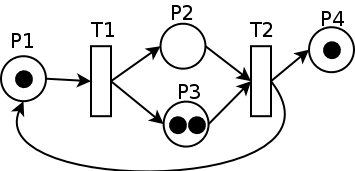
\includegraphics[scale=0.25]{petri_net.png}
\caption[]{An example of a Petri network \label{exampleNet}}
\end{figure}
Petri nets have many applications including data analysis, simulation of systems, and showing correctness of a system. The techniques we present are for the application of high level robot control. In addition to their many applications, an important advantage of Petri nets is that there are many techniques for analyzing them \cite{barrett2010architecture}. The disadvantage of Petri nets for this application is that they must be hand coded using designer knowledge of the domain. For complex tasks this is not scalable.

\subsection{The NEAT Algorithm}

The NeuroEvolution of Augmenting Topologies (NEAT) algorithm is a powerful tool for evolving the structure and weights of an artificial neural network. NEAT specifies the structure of a neural network with nodes and connection genes. It then alters the topologies of neural networks with crossover operations and mutation operations. Each gene has an innovation number associated with it which allows genomes of networks with very different structures to match up during crossover operations. Mutation operations can change the structure of a new network by addings nodes or connections between nodes. In addition to the normal evolutionary algorithm techniques, NEAT utilizes speciation to give new topological innovations time to develop \cite{neat}. Finally, NEAT starts with a uniform population of simple networks thus biasing the search towards simpler networks.

\section{Related Work}
FSA-based approaches, BDI approaches and PN-based approaches are three broadly used methods for plan designing and high-level robot control.

\subsection{Finite State Automata}

Finite State Automata (FSA) is widely and explicitly used in many robot programming languages, that support robot-control modeling. FSA-based approaches allow intuitive design of single-robot behavior model, while lacking the ability to model concurrent behaviors such as cooperation and competition between multiple agents. FSA-based approaches require manual design to come up with plans for modeling. Nevertheless, some methods have been developed that automately generate FSA-based plans \cite{kress2009temporal}.  

\subsection{Belief, Desire, Intention}

An alternative approach to the FSA-based apporach is the Belief, Desire, Intention framework (BDI). In this framework, a robot uses the current state of the environment (noted as beliefs) and a certain given goal (noted as desires) to determine an action (noted as intentions) to execute (in order to reach its goal). As an advantage over FSA-based approaches, BDI allows the designer to plan with basic behaviors in a predefined library without specifying the order. However, it is hard to develop automated planners and validation tools for BDI approaches.  

\subsection{Petri Net for High Level Robot Control}

Petri Nets can be used to describe robot behavior such as actions, action failures, action synchronization, sensing and loops. As an approach to model and analyze discrete events, Petri Nets have been used in both single robot control \cite{costelha2007modelling} and multi-robot interactions \cite{sheng2005peer}\cite{palamara2009teamwork}. The typical processes of developing plans for describing robot behavior can be classified as plan design or plan generation. Plan design, as named, is the process of hand coding behavior plans that lead to accomplishing the given task. On the other hand, plan generation, takes care of generating the solution to achieve the goal of the given task with the description of the goals and capabilities of the system. The nature of the former process is highly labored and limits the scale of use of Petri Nets, since the size and the complexity of a designed plan depends on the knowledge provided by the designers. The latter one, which automates the process, seems more appealing but is limited to simple task. Thus, neither of them has been shown to be promising to date. 

Behavior representation frameworks based on Petri Nets \cite{ziparo2011petri} has been proposed and used for high level description of single robot behaviors and concurrent behaviors. Petri Net Plans (PNPs) \cite{ziparo2011petri} are defined as a formal language for the representation of generic behaviors, which allows complex plans to be designed intuitively. It allows automated plan verification and implementation of a development environment, while being able to model coordination and collaboration for multi agents. Thus, these features allow PNPs to be an effective tool for the representation of multi-robot plans, supporting the design of cooperation. It can describe highly expressive plans for dynamic environments that are partially observable and unpredictable. The basic structures of a PNP are ordinary and sensing actions that do not occur instantly. These basic structures are then combined to describe action sequences, conditional actions, parallel actions, loops and interruption. A sub-plan is also used to represent a primitive behavior in order to achieve higher modularity in a PNP. 

Inspired by PNPs, we propose that evolved Petri Nets could be used as basic network building blocks for primitive tasks, and then to gradually build a more complex network by combining these basic network-block into a larger network.  

\section{Evolution of Petri Networks}

We propose that the Neuroevolution of Augmenting Topologies (NEAT) could be used to evolve Petri Nets. Like neural networks, Petri nets are a combination of nodes and connections (arcs) with weights on the connections. We only must modify the genome specification and the mutation operators to adapt NEAT to evolve Petri nets. With these changes NEAT becomes the PetriNEAT algorithm. The following subsections describe these changes in more detail.

\subsection{Petri Net Genes}

PetriNEAT evolves individuals that are specified by a genome. A genome contains genes of two types: nodes and arcs. Node genes can represent either places or transitions depending on a specified type. The type of node determines what other node properties will be expressed. For instance, transition nodes do not express the initial tokens trait. Alternatively, transitions and place nodes can be viewed as having their own type of gene however it was simpler to only implicitly do this. All gene values are integers with the exception of Action I.D.s which are bit strings. This allows actions to be mutated easier.

\begin{figure}
%\begin{table}
\centering
\begin{tabular}{|c|}
\hline
Node Gene\\ \hline
I.D. \\
Type \\
Initial Tokens \\
Action I.D. \\
Condition \\
\hline
\end{tabular}
\begin{tabular}{|c|}
\hline
Arc Gene\\ \hline
Place I.D.\\
Transition I.D.\\
Weight \\
 - \\
 -\\
\hline
\end{tabular}
%\end{table}
\caption{PetriNEAT uses two types of genes: node and arc genes.}
\end{figure}


\subsection{Petri Net Mutation Operators}

PetriNEAT uses very similar mutation operators to the original NEAT algorithm. The only change is that each mutation must result in a valid network. Our operators are:
\begin{itemize}
\item \emph{Mutate{\_}Add{\_}Node:} Increases the number of transitions or places in the network
\item \emph{Mutate{\_}Add{\_}Link:}  Increases connectivity of the network
\item \emph{Mutate{\_}Node:}  Changes the token count for place nodes. Changes the action associated with transitions.
\item \emph{Mutate{\_}Link:} Changes the weight of the link.
\end{itemize}

Mutations are applied when reproducing the top individuals of each species. The Mutate Add Link operator adds an arc between a random place and transition node when an offspring is created. This mutation occurs with probability 0.1. Mutating initial token counts and arc weights is done by either incrementing or decrementing with equal probabilities. These mutations occur with probability 0.1. For transition nodes, a mutation can flip bits in the action I.D. with probability 0.5. 

Mutate{\_}Add{\_}Node can happen in two different ways. The first method randomly chooses two nodes of the same type and adds a node of the opposite type between them. Then an arc is added from the first node to the new node and from the new node to the second node. The node and arc genes are initialized with random values for tokens, actions I.D.s, weights, etc. The second method chooses a random place node and creates a new transition and place node. Then arcs from the original place to the new transition and from the new transition to the new place are added. This serves to grow the size of the network more effectively.

  \begin{figure}
    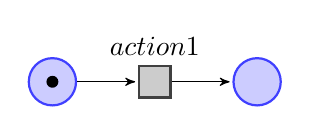
\begin{tikzpicture}[node distance=1.3cm,>=stealth',bend angle=45,auto]
  \tikzstyle{place}=[circle,thick,draw=blue!75,fill=blue!20,minimum size=6mm]
  \tikzstyle{transition}=[rectangle,thick,draw=black!75,
              fill=black!20,minimum size=4mm]
    \node [place,tokens=1,xshift=5cm] (p1){};
    \node [transition] (t1) [right of=p1, label=above:$action1$] {}  edge [pre] (p1);
    \node [place] (p2)  [right of=t1] {} edge [pre] (t1);
\end{tikzpicture}
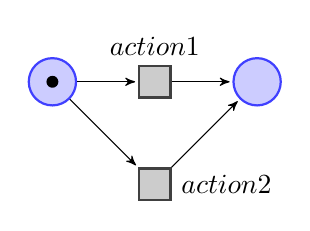
\begin{tikzpicture}[node distance=1.3cm,>=stealth',bend angle=45,auto]
  \tikzstyle{place}=[circle,thick,draw=blue!75,fill=blue!20,minimum size=6mm]
  \tikzstyle{transition}=[rectangle,thick,draw=black!75,
        fill=black!20,minimum size=4mm]
    \node [place,tokens=1] (p1){};
    \node [transition] (t1) [right of=p1, label=above:$action1$] {}  edge [pre] (p1);
    \node [place] (p2)  [right of=t1] {} edge [pre] (t1);
    \node [transition] (p3) [below of=t1, label=right:$action2$] {} edge [pre] (p1) edge [post] (p2);
\end{tikzpicture}

\caption{Adding connectivity}
\end{figure}

\begin{figure}
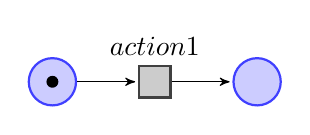
\begin{tikzpicture}[node distance=1.3cm,>=stealth',bend angle=45,auto]
  \tikzstyle{place}=[circle,thick,draw=blue!75,fill=blue!20,minimum size=6mm]
  \tikzstyle{transition}=[rectangle,thick,draw=black!75,
              fill=black!20,minimum size=4mm]
    \node [place,tokens=1, yshift=5em] (p1){};
    \node [transition] (t1) [right of=p1, label=above:$action1$] {}  edge [pre] (p1);
    \node [place] (p2)  [right of=t1] {} edge [pre] (t1);
\end{tikzpicture}
\hspace{5mm}
 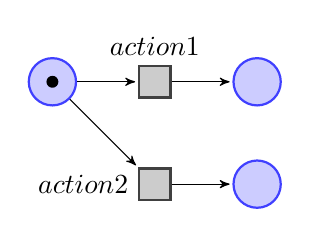
\begin{tikzpicture}[node distance=1.3cm,>=stealth',bend angle=45,auto]
  \tikzstyle{place}=[circle,thick,draw=blue!75,fill=blue!20,minimum size=6mm]
  \tikzstyle{transition}=[rectangle,thick,draw=black!75,
        fill=black!20,minimum size=4mm]
    \node [place,tokens=1] (p1){};
    \node [transition] (t1) [right of=p1, label=above:$action1$] {}  edge [pre] (p1);
    \node [place] (p2)  [right of=t1] {} edge [pre] (t1);
	\node [place] (p4) [below of=p2] {};    
    \node [transition] (p3) [below of=t1, label=left:$action2$] {} edge [pre] (p1) edge [post] (p4);
    
\end{tikzpicture}
\caption{Grow the network}
\end{figure}

\section{Methodology and Results}

\begin{figure}[b]
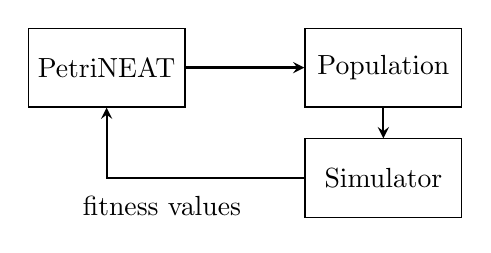
\begin{tikzpicture}

\tikzstyle{line} = [draw, -stealth, thick]
\tikzstyle{elli}=[draw, ellipse, minimum height=8mm, text width=5em, text centered]
\tikzstyle{block} = [draw, rectangle,  text width=5em, text centered, minimum height=10mm, node distance=10em]

\node [block] (population) {Population};
\node [block, below of=population, yshift=6em] (simulator) {Simulator};
\node [block, left of=population] (algorithm) {PetriNEAT};

%arrows
\path [line] (algorithm) -- (population);
\path [line] (population) -- (simulator);
\path [line] (simulator) -| node[yshift=0.5em, xshift=2em, yshift=-1.5em] {fitness values} (algorithm);
\end{tikzpicture}
\caption{Each individual is produced by the PetriNEAT algorithm and then evaluated in the simulator. The fitness values are then used to guide PetriNEAT in producing the next generation of the population.}
\end{figure}

\begin{figure} [b]
\centering
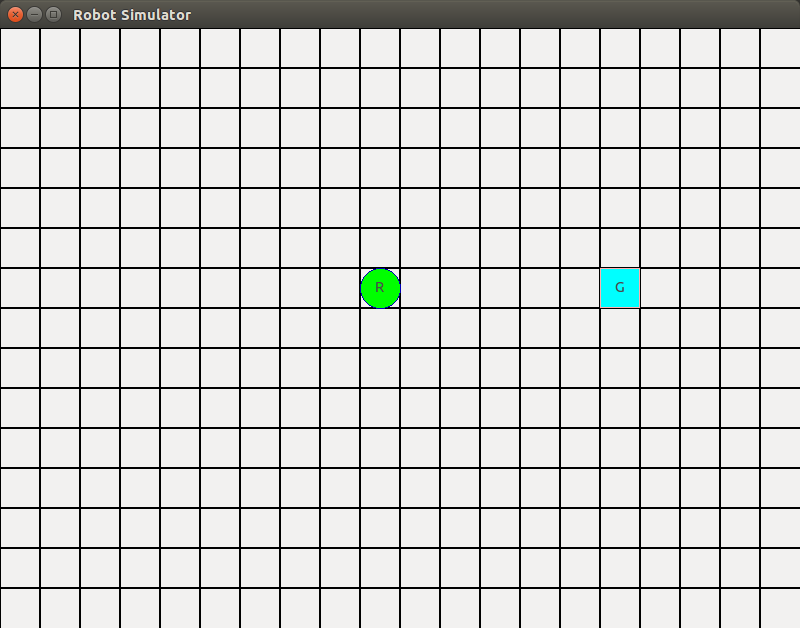
\includegraphics[scale = 0.4, trim = 100mm 90mm 20mm 70mm, clip = true]{robot_sim.png}
\caption{Visualization of the simulator. A grid world with a robot represented by a green circle and a goal represented by a sky blue square.}
\label{fig:grid}
\end{figure}

In this section we discuss the setup for the environment as well as the two different approaches that were taken to evaluate our hypothesis. 
%The application we chose to evolve Petri Nets for was Robot Control; 
Our target domain was a simple grid world simulator (shown in Figure~\ref{fig:grid}) that we designed.
%to accomplish our goal we created a simulator that consisted of a really simple grid world shown in Figure~\ref{fig:grid}. 
This simulator consists of a robot represented by a green circle and a goal that must be reached represented by a blue square. The actions that the robot could take, the ways in which the robot could interact with the world and the fitness function used to evaluate the actions taken were different in both approaches. In the subsections below we describe what both approaches consist of and the values of the environment parameters used to run the experiments.

The setup for the environment consisted of the population size, the maximum number of generations, the starting genome, the probabilities for the mutation operators, the maximum number of actions to execute in the Petri net, and the parameters in the fitness function. Since most of the parameters change depending on the approach, they will be discussed in the proper subsections. The only parameter that was held constant in both approaches was the maximum number of actions that the robot could take while executing a Petri net, which corresponds to the number of transitions fired. We set this value to 50 because the distance between the goal and the initial robot position was a maximum of 10 on each axis for our trials. Since mutations occur randomly we cannot guarantee that there will be a solution, which is why we need to set a maximum number of actions to halt the execution of the network.

%\begin{figure}
%\[fitness = \frac{2^{goalReached}}{1.0 + distance + actions}\]
%\caption{The fitness function used in the first approach. goalReached is a binary flag, distance is the final distance from the goal multiplied by 3, actions is the number of actions taken by the robot to reach the goal.}
%\label{eq:fitnessFunction}
%\end{figure}

\subsection{First Approach}
\label{subsec:firstApproach}
As stated above, both approaches consist of the robot reaching the goal. For this approach the actions that the robot could take were: Move Right, Move Up, Move Left and Move Down. These actions are represented by transitions; whenever the transition fires the action is executed. The goal was always in a fixed position, so we evolved the network to come up with actions to reach that position as efficiently as possible. In order to determine how well was the task executed we used the fitness function:

\begin{equation}
fitness = \frac{2^{goalReached}}{1.0 + distance + actions}\label{eq:fitnessFunction}
\end{equation}
 where goalReached is a binary flag, distance is the final distance from the goal multiplied by 3, actions is the number of actions taken by the robot to reach the goal.
% shown in Figure~\ref{eq:fitnessFunction}. 
 With this approach and conditions we were able to find a solution pretty quickly, as every action taken directly affects the fitness value generated and the task is quite simple. We tested this approach with a population size of 256, a maximum of 100 generations, a starting genome shown in Figure~\ref{fig:genome} and the mutation probabilities shown in Figure~\ref{tab:probabilities}. 

\begin{figure} [b]
%\begin{table}
\centering
\begin{tabular}{|l c r|}
\hline
Mutation probabilities & & \\ \hline
Mutate Add Node & = & 0.0\% \\
Mutate Add Link & = & 0.0\% \\
Mutate Node & = & 0.0\% \\
Mutate Link & = & 0.0\% \\
Mutate Condition & = & 0.0\% \\
\hline
\end{tabular}
%\end{table}
\caption{Mutation probabilities for the net.}
\label{tab:probabilities}
\end{figure}

\begin{figure} [h]
\centering
\caption{Starting genome used for the first approach. Two places with one token and a transition between them that consumes and produces one token. The action associated with the transition is ``Move Right"}
\label{fig:genome}
\end{figure}

%The results found for this approach were what we hoped for, 
Using this approach, we were able to evolve the networks correctly and generate different plans that solved the task at hand. Figures~\ref{fig:pn1_1} and ~\ref{fig:pn1_2} show us examples of Petri nets evolved to solve the task where the goal is six steps to the right of the starting position. An interesting point to notice about Figure~\ref{fig:pn1_1} is that we can see some of the mutations that arrive at different solutions with the same structure but different weights and initial markings, while in Figure~\ref{fig:pn1_2} we can see examples of the different types of resulting architectures. Figure~\ref{fig:pn1_3} shows us two different Petri nets that solve a different task where the goal is down and to the left. 

While this approach proves that we can evolve Petri net plans for these kind of tasks, the approach is still very constrained. First of all, the robot can only execute actions in the world and the plan only succeeds if there are no more possible transitions (actions) when the goal was reached. In the real world a robot has sensors and we may want to execute an action only if a certain condition is met. Also, we would like to determine if the goal has already been reached. Additionally, while the actions described here can easily be performed by most robots, this is not the usual way in which they work. In order to tackle all of these issues we changed the simulator and came up with the second approach described below. 

\begin{figure} [h]
\centering
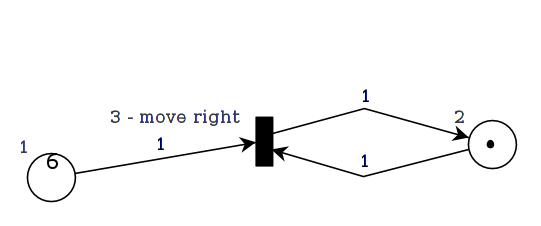
\includegraphics[scale=0.3, trim = 0 5mm 0 30mm, clip = true]{PetriNet_1_1}
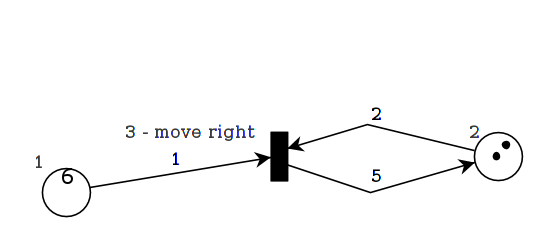
\includegraphics[scale=0.3, trim = 0 5mm 0 35mm, clip = true]{PetriNet_1_2}
\caption{Example Petri nets generated to solve the task where the goal is six steps to the right. We can see both have the same architecture but different markings and weights.}
\label{fig:pn1_1}
\end{figure}

\begin{figure} [t]
\centering
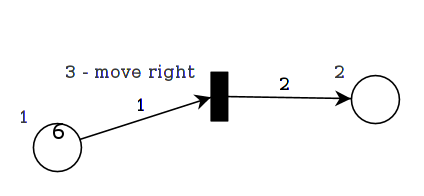
\includegraphics[scale=0.3, trim = 0 5mm 0 20mm, clip = true]{PetriNet_1_3}
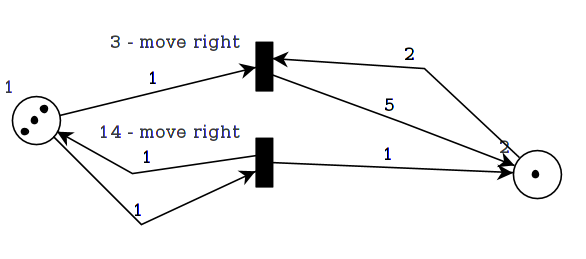
\includegraphics[scale=0.3, trim = 0 5mm 0 10mm, clip = true]{PetriNet_1_4}
\caption{Example Petri nets generated to solve the task where the goal is six steps to the right. Both networks have completely different architectures.}
\label{fig:pn1_2}
\end{figure}

\begin{figure} [h]
\centering
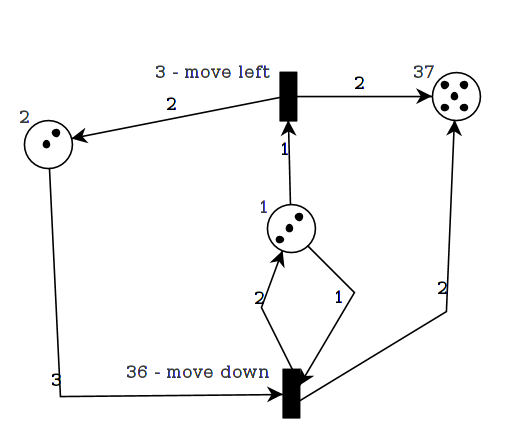
\includegraphics[scale=0.3, trim = 0 5mm 0 20mm, clip = true] {PetriNet_2_1}
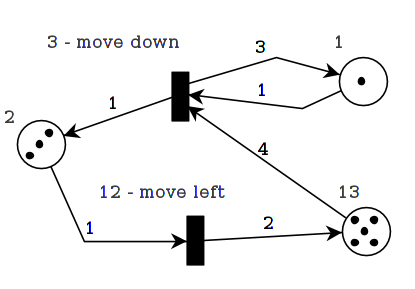
\includegraphics[scale=0.3, trim = 0 10mm 0 20mm, clip = true] {PetriNet_2_2}
\caption{Example Petri nets generated to solve the task where the goal is down and to the left.}
\label{fig:pn1_3}
\end{figure}

\subsection{Second Approach}
The second approach that we took aimed to address the problems discussed at the end of section ~\ref{subsec:firstApproach}. Additionally, with this approach we wanted to solve the task where the goal is at an arbitrary position within the grid. The first important change we made was to have different actions: Rotate 90 degrees, Rotate 180 degrees, Rotate 270 degrees and Step Forward. We gave the robot a direction which he was facing and gave him actions to rotate to the left and to step forward. By doing this, we can achieve all of the possible movements that could be executed in our first approach. The advantage is that now we allowed our robot to sense the world in two different ways: we can halt whenever we identify that we're at the goal and we can see if the goal is within the field of view of the robot. In order to keep things simple we gave the robot a 90 degree FoV, which allowed us to cover one fourth of the grid depending on the direction the robot is facing. 

With the first approach, the only way to solve the new kind of task in which the goal is at an arbitrary position would be to move through every single position in the grid. On the other hand, with the second approach we can think of many useful solutions, e.g. rotating and only moving forward if you're looking at the goal. In order to determine that this approach was correct we first evolved the network for the goal in a fixed position.

While we started out trying the same parameters as the ones used in the first approach, we had to make some changes in order to evolve the network properly. The most important change we made was the way in which the fitness function worked; instead of calculating a fitness value at the end of the execution, we gave a reward (or punishment) every time the robot executed an action. Since we were working only with positive fitness values we gave the robot a starting fitness of 10.0. The behavior/reward rules are as follows:
\begin{itemize}
\item Whenever an action is taken: subtract 0.02 from the fitness value.
\item If the distance was decreased by taking this action: add 0.15 to the fitness value.
\item If the distance was increased by taking this action: subtract 0.15 from the fitness value.
\item If the robot was not facing the goal and this action caused him to face the goal: add 0.05 to the fitness value.
\item If the robot was facing the goal and this action caused him to turn away from it: subtract 0.05 from the fitness value.
\end{itemize}

The reward/punishment values are based on the starting fitness and the fact that there's a maximum of 50 actions we're allowing the robot to execute. Additionally, we wanted the distance to have a higher impact than facing the goal and both of these things to have a higher impact than taking an additional actions. 

The transitions were changed by adding a condition to them and could only fire if it was met. We currently have two types of conditions, the first one is always true, i.e. no condition, the second one corresponds to the robot facing the goal. We included the ``no condition" condition in order to be able to mutate the condition related to a transition. The ``goal reached" sensor was generated by halting the execution if the robot position was the same as the goal position. 

\begin{figure}
\centering
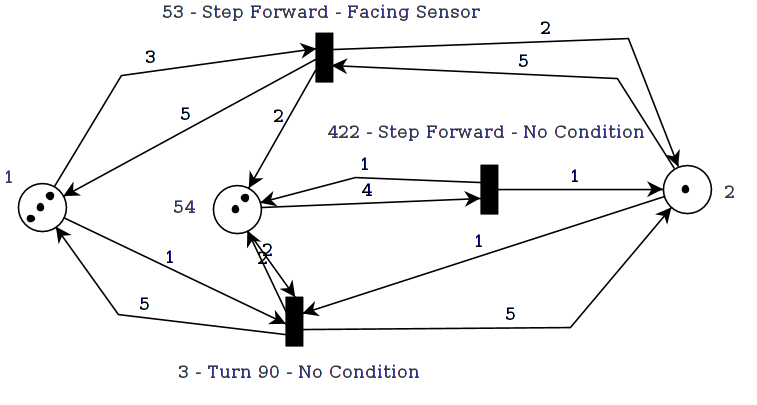
\includegraphics[scale=0.3, trim = 0 5mm 0 0, clip = true] {PetriNet_3_1}
\caption{Example Petri net generated to solve the task where the goal is down and to the left with the second approach.}
\label{fig:pn2_1}
\end{figure}

For the other parameters, the starting genome used was the same as the one in the first approach, with the action being ``Turn 90 degrees" instead of ``Move right". We first tried using the same population size and maximum number of generations which did yield good results. However, by increasing the population size to 2048 and the maximum number of generations to 1000 we were able to find solutions which solved the task in a few less steps. It's worth noting that while this might sound like a big change the solutions were still found in a matter of a few seconds (around 8-10) compared to the 2 seconds that it took using a population size of 256 and a maximum of 100 generations. Figure~\ref{fig:pn2_1} shows a sample solution found for the same task as Figure~\ref{fig:pn1_3} using this approach. While it iss evident that the network is more complex than the ones found for the first approach, we also know that we're able to accomplish more with this kind of representation.

We are currently working on a way to generalize the solution for the goal at an arbitrary position. Our insight is that we can generate multiple simulations with the goal at different positions and then get an average fitness value that can be used for the organism. However, we haven't finished implementing this and therefore we can't confirm that we can evolve a Petri net that reaches a goal at an arbitrary position. While we were not able to confirm our hypothesis for these types of tasks, this approach still brings the benefits of evolution by changing our fitness when an action is taken and adding conditions to the transitions in the network. 

\section{Discussion and Future Work}
The major contribution of this paper is that we show that it is possible to evolve Petri nets for a specific task, which to the best of our knowledge has not been attempted by anyone so far. While we were not able to do this for a more complex task such as the goal being in an arbitrary position in the grid, we give some intuition as to why should this work. Additionally, we show a way in which Petri nets can be used for high level robot control (i.e. using transitions as actions to execute) as well as a way to incorporate sensors into the network. 

It's important to note that while the tasks we show here are pretty simple they can potentially be used as building blocks for more complex tasks. As an example, we could have a more complex task which consists of approaching a ball and the kicking it, where the task shown in this paper could be used to approach the ball. This could also be beneficial since we could use the building blocks as actions for more complex tasks and then apply our mutation operators on this actions to evolve for our complex task. 

We believe that the results found here could have a great impact on the way that robotic plans are made; we would only need a fitness function for the behavior we want to see instead of a detailed plan that we want the robot to perform.  This could also potentially help the robot be more autonomous by coming up with solutions for new problems and adapting to new situations. However, there's still much work to be done in this area to see how viable this evolution mechanisms can be. We list some of the future work avenues that we consider essential below:

\begin{itemize}
\item Finish the second approach by evaluating the network for an arbitrary goal position.
\item Add more actions, sensors and obstacles to the world.
\item Explore different kind of tasks with different reward functions that do not necessarily depend on a distance metric.
\item Add cross over operations to the evolutionary algorithm.
\item Explore different mutation operators.
\item Add methods to combine Petri nets into hierarchies, i.e. ways to use the building blocks described above.
\item Use the reachability graph to simplify a network for which a solution has been found.
\end{itemize}

\section{Conclusion}

In this paper, we have shown that it is possible to evolve Petri nets. With the experiments, we showed that for Petri nets, weights of nodes, markings of nodes, and structure of the network can adapt to improve network fitness. By setting an appropriate fitness function, it is possible for the networks to be evolved through properly defined mutation operations and to solve certain given task. It has also been shown that using mutations that create simple structures, higher level actions can be represented using the simple structures as building blocks. Moving forward we hope to further generalize our method to make it applicable for a wider range of robotics and Petri net problems.

\bibliographystyle{plain}
\bibliography{project}

\end{document}